
\begin{figure*}[htb]
  \colorrule{grey3}{\textwidth}{1.5pt}
  \center
  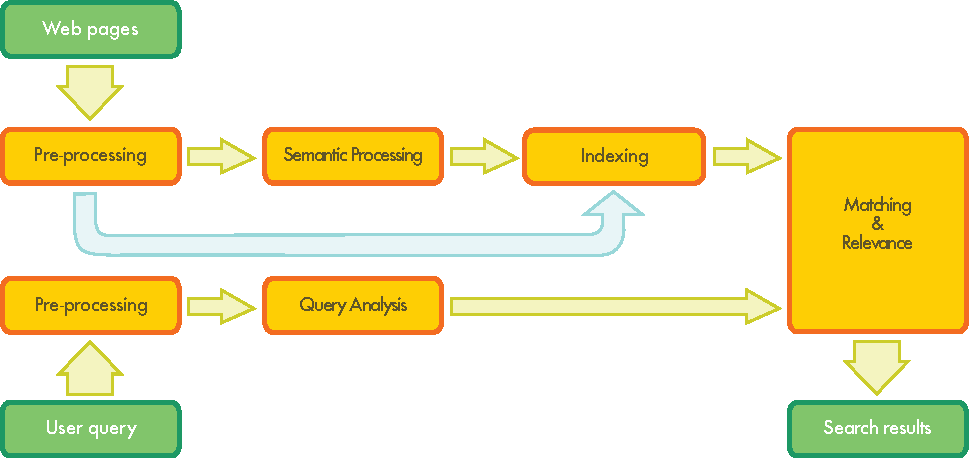
\includegraphics[width=\textwidth]{../_media/english/web_search_architecture}
  \caption{Web search}
  \label{fig:websearcharch_en}
  \colorrule{grey3}{\textwidth}{1.5pt}
 \end{figure*}

Searching on the web, in intranets, or in digital libraries is probably the most widely used and yet underdeveloped Language Technology today. The search engine Google, which started in 1998, is nowadays used for about 80\% of all search queries world-wide. In 2006, the verb \emph{googlovať/googliť} very narrowly missed being included in the first volume of the new Dictionary of Contemporary Slovak Language (\emph{Slovník súčasného slovenského jazyka}), a fact that is over being used to reproach the dictionary authors for. Neither the search interface nor the presentation of the retrieved results have significantly changed since the first version. In the current version, Google offers a spelling correction for misspelled words and also, in 2009, incorporated basic semantic search capabilities into their algorithmic mix\footnote{\url{http://www.pcworld.com/businesscenter/article/161869/google_rolls_out_semantic_search_capabilities.html}}, which can improve search accuracy by analysing the meaning of the query terms in context. The success story of Google shows that with a lot of data at hand and efficient techniques for \underbar{indexing} these data, a mainly statistically-based approach can lead to satisfactory results. 

However, for a more sophisticated request for information, integrating deeper linguistic knowledge is essential. In research labs, experiments using machine-readable \underbar{thesauri} and \underbar{ontological language resources} like WordNet, have shown improvements by allowing to find a page on the basis of synonyms of the search terms, e.g. \emph{jadrová}, \emph{atómová} and \emph{nukleárna energia} (nuclear, atomic and nuclear energy) or even more loosely related terms. 

\boxtext{The next generation of search engines will have to include much more sophisticated Language Technology}

The next generation of search engines will have to include much more sophisticated Language Technology. If a search query consists of a question or another type of sentence rather than a list of keywords, retrieving relevant answers to this query requires an analysis of this sentence on a syntactic and semantic level as well as the availability of an index that allows for a fast retrieval of the relevant documents. For example, imagine a user inputs the query ‘Give me a list of all companies that were taken over by other companies in the last five years’. For a satisfactory answer, syntactic \underbar{parsing} needs to be applied to analyse the grammatical structure of the sentence and determine that the user is looking for companies that have been taken over and not companies that took over others. Also, the expression \emph{last five years} needs to be processed in order to find out which years it refers to. 

Finally, the processed query needs to be matched against a huge amount of unstructured data in order to find the piece or pieces of information the user is looking for. This is commonly referred to as \underbar{information retrieval} and involves the search for and ranking of relevant documents. In addition to generating a list of companies, we also need to extract the information that a particular string of words in a document refers to a company name. This kind of information is made available by so-called \underbar{named-entity recognisers}. 

Even more demanding is the attempt to match a query to documents written in a different language. For \underbar{cross-lingual information retrieval}, we have to automatically translate the query to all possible source languages and transfer the retrieved information back to the target language. The increasing percentage of data available in non-textual formats drives the demand for services enabling \underbar{multimedia information retrieval}, i.e., information search on images, audio, and video data. For audio and video files, this involves a \underbar{speech recognition} module to convert speech content into text or a phonetic representation, to which user queries can be matched.

In Slovakia, there were several different small and medium enterprises (SMEs) developing search technologies, or search technologies developed by Czech SMEs were used. The first Slovak search engine taking Slovak morphology\footnote{Developed at the Faculty of Mathematics and Physics, Charles University, Prague.} into account was \emph{morfeo.sk}, run by the internet portal \emph{centrum.sk}, which started to provide a fulltext search of the \emph{.sk} domain webpages in 2003. It used lemmatization and morphology annotation to look for inflected words in order to be able to provide the user with more relevant results than those including the basic forms of the words. It also included fuzzy search possibilities and search by synonyms. By 2009 the number of indexed pages was over 117 million. Since that time, Google has already included Slovak morphology support and surpassed the number of the indexed pages and \emph{centrum.sk} has switched to a customised Google Search.

One of the enterprises engaged in this field is Forma s.\,r.\,o.\footnote{\url{http://www.forma.sk/}}, a company that developed three linguistic modules: speech check, hyphenator, lemmatiser and thesaurus, on the basis of data obtained from the Ľ. Štúr Institute of Linguistics of the Slovak Academy of Sciences. The company also developed separate programs for full-text Slovak search and still operates online versions of some older dictionaries. 

Focus on development for search technologies lies in providing add-ons and advanced search engines for special-interest portals by exploiting topic-relevant semantics. Due to the still high demands in processing power, such search engines are only economically usable in relatively small text corpora. The processing time easily exceeds that of a common statistical search engine as e.g., provided by Google by a magnitude of thousands. These search engines also have a high demand in topic-specific domain modelling, making it infeasible to use these mechanisms on a web scale.

Research in this field is mainly performed by the Institute of Informatics of the Slovak Academy of Sciences, which started to deal with the processing of written natural language in 2006. At the same time, WIKT\footnote{\url{http://conference.ui.sav.sk/wikt2010/}} workshops, containing several articles or even entire sections dedicated to the processing of Slovak language in each year have been initiated. Since 2006, the research in the Institute of Informatics in cooperation with Pavol Jozef Šafárik University in Košice has been mainly performed within the NAZOU\footnote{\url{http://nazou.fiit.stuba.sk}} project aimed at the development of the tools for obtaining, processing, organizing and presenting Internet information. Job offers represented a specific application with the tools having been tested on Slovak job offers as well.  The Institute prepared an analysis of processing texts in Slovak \cite{laclavik2007a} and, at the same time, Ontea\footnote{\url{http://ontea.sourceforge.net/}}, a tool for extracting of information \cite{laclavik2007b,laclavik2009} was developed. The tool was later integrated with the tools for language identification \cite{vojtek2006} and lemmatisation \cite{krajci2007}.

Ontea works on the basis of searching for patterns, which can either be linguistically dependent patterns, such as use of prepositions and sentence structure, but also simpler patterns, such as use of capitals and abbreviations e.g. s. r. o. and a. s. for searching for businesses, \emph{SK}, \emph{SKK}, \emph{EUR}, \emph{EURO}, \emph{\euro} for price searching, or abbreviations of Slovak first names for searching for people in a text. A principle is applicable to various languages, but the patterns have to be made for a specific language, e.g. Slovak.  At the present, the Ontea tool is being improved for use in the processing of e-mail communication. The system was tested within the AIIA project\footnote{\url{http://aiia.ui.sav.sk/}} \cite{laclavik2010} on Slovak e-mails from the Anasoft company and SANET association. Ontea not only uses the patterns, but also dictionaries (gazetteers) as well as their combinations in order to extract and identify entities in a text. Since the use of dictionaries (but also some patterns) can cause problems with the identification of an entity that is in other than basic form, use of lemmatiser seems to be appropriate. Since the entities are mostly of a nomenclatural nature, such as people, locations, product names, names of projects or services, they are difficult to be lemmatised. Although the problems have not yet been successfully resolved, they could be settled by a new method with the combination of dictionaries, character based tokenization, lemmatisation, and verification of an entity in a dictionary.

The extraction of entities using patterns was also used in an experiment with large group of data, when Slovak websites were processed with an aim of extraction of geographical data (Slovak addresses) and their subsequent finding \cite{dlugolinsky2010}.
